%
% File naaclhlt2016.tex
%

\documentclass[11pt,letterpaper]{article}
\usepackage{naaclhlt2016}
\usepackage{times}
\usepackage{latexsym}
\usepackage{bm}
\usepackage{mathtools}
\usepackage{csquotes}
\usepackage{url}
% \usepackage{hyperref}
\usepackage{subcaption}

\usepackage{array}



\naaclfinalcopy % Uncomment this line for the final submission
\def\naaclpaperid{***} %  Enter the naacl Paper ID here

% To expand the titlebox for more authors, uncomment
% below and set accordingly.
% \addtolength\titlebox{.5in}    

\newcommand\BibTeX{B{\sc ib}\TeX}


\title{Constructing narrative using a generative model and continuous action policies}

% Author information can be set in various styles:
% For several authors from the same institution:
% \author{Author 1 \and ... \and Author n \\
%         Address line \\ ... \\ Address line}
% if the names do not fit well on one line use
%         Author 1 \\ {\bf Author 2} \\ ... \\ {\bf Author n} \\
% For authors from different institutions:
% \author{Author 1 \\ Address line \\  ... \\ Address line
%         \And  ... \And
%         Author n \\ Address line \\ ... \\ Address line}
% To start a seperate ``row'' of authors use \AND, as in
% \author{Author 1 \\ Address line \\  ... \\ Address line
%         \AND
%         Author 2 \\ Address line \\ ... \\ Address line \And
%         Author 3 \\ Address line \\ ... \\ Address line}
% If the title and author information does not fit in the area allocated,
% place \setlength\titlebox{<new height>} right after
% at the top, where <new height> can be something larger than 2.25in
\author{Emmanouil Theofanis Chourdakis \and Joshua D. Reiss\Thanks{Correspondence should be sent to the first author. This paper has been sponsored by RPPtv Ltd.}  \\Queen Mary University of London\\ Mile End Road, E1 4NS\\London, UK \\ \texttt{\{e.t.chourdakis,joshua.reiss\}@qmul.ac.uk}}

%Centre for Digital Music, Queen Mary University of London, London, UK, \\{\tt \{e.t.chourdakis, joshua.reiss\}@qmul.ac.uk}}}

\date{}

\begin{document}

\maketitle

\begin{abstract}
This paper proposes a method for learning how to generate narrative by recombining sentences from a previous collection. Given a corpus of story events categorised into 9 topics, we approximate a deep reinforcement learning agent policy to recombine them in order to satisfy narrative structure. We also propose an evaluation of such a system. The evaluation is based on coherence, interest, and topic, in order to figure how much sense the generated stories make, how interesting they are, and examine whether new narrative topics can emerge.

\end{abstract}

\section{Introduction}

 In this work reinforcement learning is used in conjunction with a shallow generative artificial neural network (ANN) to generate novel stories. First, a SkipGram  \cite{mikolov2013efficient} based model is derived that generates parts of the narrative in a local neighbourhood (a few consecutive events at time). An artificial agent is then used to extend its use to the whole narrative while globally adhering to the story structure learned by that model.

\section{Previous Work}

Data-driven approaches for story generation can be found in \cite{mcintyre2009learning,li2013story}. In \cite{mcintyre2009learning}, the authors present an end-to-end system to generate stories by deriving models of interest and coherence and a generator that creates stories by consulting a knowledge base of story elements and their possible interactions. They improved their work in \cite{mcintyre2010plot} by generating stories with genetic algorithms instead of specified models for interest. In \cite{li2013story}, the authors recombine events found in a story corpus with a planning algorithm to create novel stories which consist of events in the form of simple sentences. Their novelty relies on that they crowd-source the corpus in natural language sentences and do not need to provide a pre-defined knowledge base. In that work, they use paraphrase identification using weighted dependencies \cite{lintean2009paraphrase} in order to group similar events which they use to construct graphs of narration and a planning algorithm to generate new stories. \cite{riedl2016using} use that work together with Reinforcement Learning in order to teach artificial agents human values.  Deep Reinforcement Learning has been explored in the context of natural language generation before in the context of text-based games. In \cite{narasimhan2015language} the authors introduce a recurrent neural network which they call LSTM-DQN, to characterise the states of the worlds of text-based Multi-User Dungeon games. They then use Deep Q-learning \cite{mnih2015human} to learn optimal policies for such games. In \cite{he2015deep} the authors introduce a novel type of ANN called Deep Reinforcement Relevance Network which allows for separate ANNs to use for the states and actions of the agents allowing actions of arbitrary number or complexity to be taken by the agent. In this work we use such a network with an actor-critic method and devise a data driven approach for story generation to learn how to construct narratives from a collection of stories.







\section{Methodology}





\subsection{Event Representation}
\label{section:eventrepresentation}

We used 519 stories from the \textsc{Scheherazade} system \cite{li2013story}\footnote{\url{http://boyangli.co/openstory.php}} which contains simple stories pertaining to 9 topics with an average length of 7-16 events per story per topic. These stories consist of simple sentences, each describing a single event. Using the Stanford NLP parser, we extract the Universal Dependencies \cite{chen2014fast,nivre2016universal} of each sentence as a list of relations in the form $rel(head, modifier)$ where $rel$ is the relation type and $head$, $modifier$ are literals. We further lemmatize each $head$ and $modifier$ using WordNet \cite{miller1995wordnet} in order to reduce the total number of literals we have to deal with. Narratives are sequences of  events which in turn are simple sentences that describe a character action or a stative. We use universal dependencies  and a shallow ANN in order to derive a useful and compact representation for each event.  Having derived a set of all the dependencies found in the corpus each event is represented as a vector $\bm v_k$ of the form $[H_{dep1}\ H_{dep2}\ \dots M_{dep1}\ M_{dep2}]^T$ where $H_{dep}$ corresponds to the head of dependency ${dep}$,  $M_{dep}$ to the modifier and each of those elements can take as values an integer that serves as the index for the literals found in the corpus.


After we extract a vector $\bm v_k$ for each event $k$ in our corpus, we use an ANN to learn a compact representation of our events such that two similar events have similar representations. Instead of measuring grammatical similarity as in \cite{li2013story} we consider as similar events the ones that are used in a similar context. For this we use a model similar to the SkipGram \cite{mikolov2013efficient}. This model derives a low-dimensional fixed-length representation space that maps events that are used similarly, close in that space thus implicitly "grouping" them together. It also gives probabilities of each event happening, based on previous events. The SkipGram model can be seen in Figure \ref{figure:model_skipgram}.

Choosing such a model allows us to capture relations between neighbouring events, in a similar way to that of the original SkipGram that captures analogies of words in language. We can then use these learned relations to generate events that satisfy them and thus create "coherent" narratives. It also allows us to implicitly group events. This means that, in the process of generating a narrative, when choosing on an event to include, we do have a probability of including a different, but similar, event. Finally, we can use it with events not found in the corpus it has been trained with. As long as we can feed it a vector representation of the new event it will be mapped close to similar events in the corpus.  We will see that by using the model generatively to predict the context from a starting event we can already make sensible narratives. 

\subsection{Generative Model}

In Section \ref{section:eventrepresentation} we introduced our SkipGram Model. This model has been trained to give an approximation of the context of an event, given that event. The context of an event in our case consists of the events that immediately surround it. By starting from a random event that can begin a narrative, the model gives the probability of the next event. An example of a narrative generated can be seen in Figure \ref{figure:story_generativemodel}. Generating narratives this way, while it appears adequate, suffers from a serious limitation.  Since the model is trained on an event and its immediate surroundings, it is not possible to capture longer distance dependencies in the narrative. In other words, we cannot interrupt a coherent sequence of events and come at it later so the model is "forced" to keep very close to the corpus in order to maintain coherence. 

\subsection{Deep Reinforcement Learning}
\label{section:trainingtheagent}

    
    Reinforcement learning is the field that studies how an abstract mathematical entity, called an \emph{agent}, can interact with an environment $\mathcal{E}$ in order to maximise a numerical quantity \cite{sutton1998reinforcement}. We call an instance of the environment at time $t$ a \emph{state} $s_t$, the quantity to maximise a \emph{utility} $U_t$. The agent interacts with the environment by executing a series of \emph{actions} $a_i$ and receiving a series of immediate \emph{rewards} $r_t$. The utility $U_t$ is related to the immediate rewards $r_t$ by the expression: $U_t = \sum_{n=1}^{t}r_n$. The series of actions the agent takes based on the state of the environment is modelled by a \emph{policy} $\pi$. The policy can be seen as a probability distribution $\pi(a_t = a_i | s_t)$. The problem of reinforcement learning therefore is to find a policy that maximises the utility for the agent in a given environment. In order to generate policies, RL algorithms usually approximate a \emph{value function} $V(s_t)$ or an \emph{action-value function} $Q(s_t, a_t)$. $V(s_t)$ gives a measure of how beneficial is for the agent to exist at the state $s_t$ and $Q(s_t, a_t)$ how beneficial it is for the agent to be at state $s_t$ and execute action $a_t$. Deep Reinforcement Learning (DRL) approximates $Q$, $V$,  $\mathcal{E}$, or $\pi$ with a Deep Neural Network. A popular approach for training agents works by suggesting an action $a_t$ using a model called an \emph{actor} and evaluates it using a model called a \emph{critic}.   The method we use in this work is called Deep Deterministic Policy Gradient \cite{lillicrap2015continuous} with the actor and critic models being the deep neural networks that appear in Figures \ref{figure:model_actor} and \ref{figure:model_critic} respectively. The model of the critic is inspired by the Deep Reinforcement Relevance Network given in \cite{he2015deep}. The actor approximates an event to be included in the narrative and the critic evaluates it based on the current state of the narrative. The state of the narrative is at every point a simple concatenation of the embeddings (as given by the hidden layer in \ref{figure:model_skipgram}) of the events included in that narrative until that point. At every step the reward is calculated based on the distance of the expected action-event  to the selected event so that it awards adding events to the narrative when those are close to the ones we expect to see, and punishes by a small amount unexpected events. Punishing unexpected events might appear counter-intuitive at first glance since story generation systems are expected to generate unexpected events. This is compensated by the stochastic nature of policies found by actor-critic methods which will also assign a small probability to an unexpected event happening.  
    
\section{Evaluation}

In order to evaluate the system's capability to generate interesting narratives human evaluation is necessary. Towards this goal, an evaluation experiment has been designed which is based on similar evaluation approaches found in data-driven story generation approaches \cite{li2013story,mcintyre2010plot} and asks 20 subjects to evaluate 40 narratives from which 10 are from our corpus of human-made narratives, 10 narratives generated by randomly combining events from the corpus, 10 are narratives generated by the SkipGram Model given in Figure \ref{figure:model_skipgram} and 10 by the DDPG agent. Each subject evaluates 8 narratives based on number of edits (rearranging, deleting, or adding new events) required to make the narrative more coherent, interest rated on a scale from 1 to 5 (1 being "Not at all interesting" and 5 being "Very Interesting") as well as asked to give one word that better describes the topic of the narrative. This last task can helps us figure out whether new topics emerge from our system by combining events from different topics. Since this is work in progress, we lack experiment results. In the absence of human evaluation results we could do some qualitative examining of generated narratives. Figures \ref{figure:story_corpus} and \ref{figure:story_corpus2} show narratives found in our original corpus and in Figures \ref{figure:story_generativemodel} and \ref{figure:story_ddpg} narratives generated by the generative model and the DDPG agent respectively. We can see that the narrative in \ref{figure:story_generativemodel} tries to follow the narrative found in \ref{figure:story_corpus2} however it deviates in its conclusion. Instead of kneeling in front of Sally and proposing, the narrative ends with John kissing Sally. An important note here is that for the most first part of the narrative, the generative model followed almost exactly the story found in the corpus. This is a weakness of the model that arises from learning relations only between neighbouring events. A more interesting narrative is the one found in \ref{figure:story_ddpg}. This narrative combines events from the narrative in Figure \ref{figure:story_corpus}, the one in \ref{figure:story_corpus2}, as well as others found in the corpus. Narratives generated by the DDPG agent tend to explore more events while narratives generated by the generative model tend to stick to the corpus.
 
\begin{figure}[h!]
    \centering
    \begin{subfigure}[b]{0.4\textwidth}
        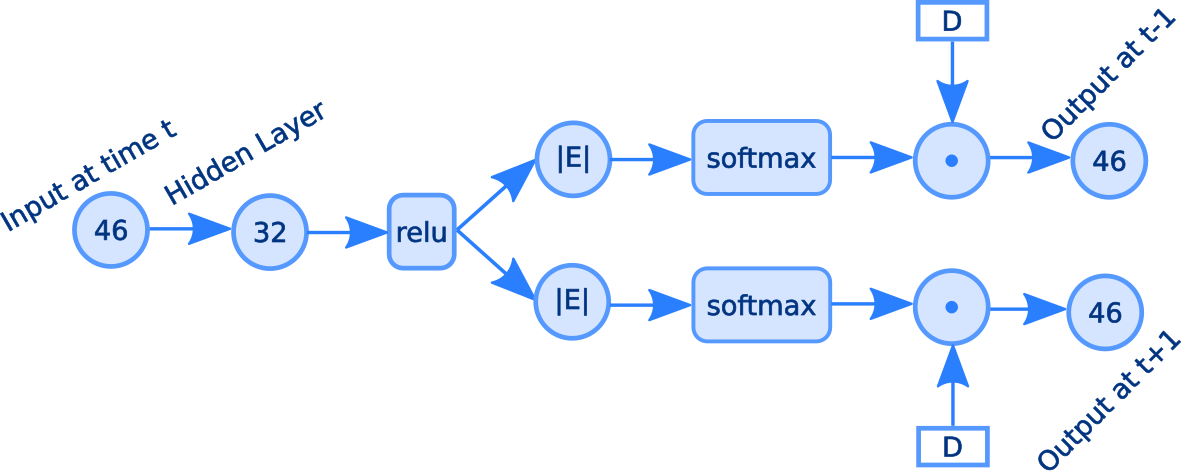
\includegraphics[width=\textwidth]{softmax}
        \caption{\small SkipGram model}
        \label{figure:model_skipgram}
    \end{subfigure}    
    \begin{subfigure}[b]{0.35\textwidth}
        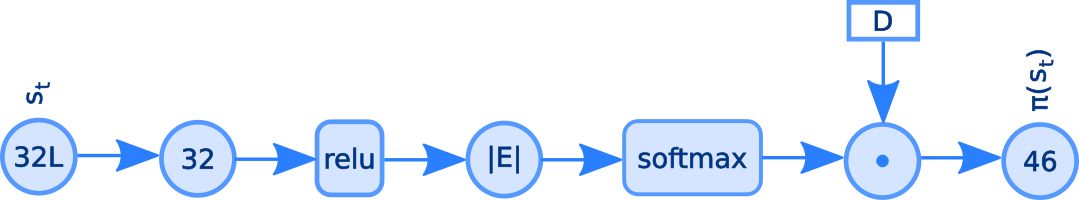
\includegraphics[width=\textwidth]{actor}
        \caption{\small actor}
        \label{figure:model_actor}
    \end{subfigure}
    ~ %add desired spacing between images, e. g. ~, \quad, \qquad, \hfill etc. 
      %(or a blank line to force the subfigure onto a new line)
    \begin{subfigure}[b]{0.35\textwidth}
        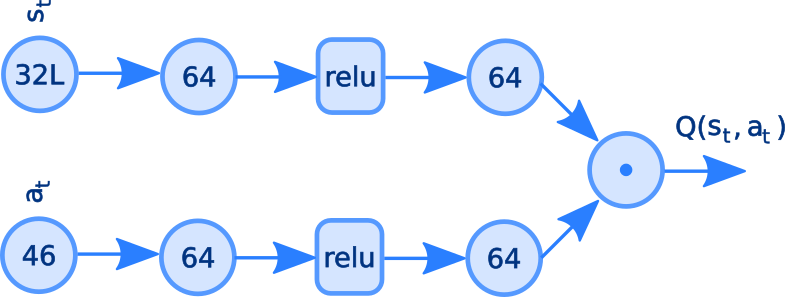
\includegraphics[width=\textwidth]{critic}
        \caption{\small critic}
        \label{figure:model_critic}
    \end{subfigure}
    
    \caption{\small The Skipgram model, and the models for the actor and the critic. Circles represent fully connected neuron layers with the number of neurons being the number inside the circle. The smoothed rectangles represent the activation functions with \texttt{relu} being the linear rectifier and \texttt{softmax} a softmax output. $|E|$ is the number of events in our database, and $D$ the narrative corpus as a matrix of features. The dot symbolises the dot product. $L$ is the number of the events making up the narrative, $\pi(s_t)$ the policy at state $s_t$, $Q(s_t, a_t)$ the state-action value for the policy $\pi$.}
    
\end{figure}

\begin{figure}[h!]
    \centering
    \begin{subfigure}[b]{0.5\textwidth}
    \blockquote{
        \textit{
        \small
        John loved Sally
        John wanted to marry Sally
        John bought an engagement ring
        John took Sally to the park
        John and Sally enjoyed a picnic
        John got down on one knee
        John presented the ring to Sally
        Sally started to cry
        John asked Sally to marry John
        Sally agreed
        Sally put on the ring
        John and Sally hugged
        }
    }



    
        \caption{An example narrative from the corpus.\vspace{0.2in}}% which gives a reward of $0.69$. The model has been trained using the ``proposal'' corpus.}
        
        \label{figure:story_corpus}    
    \end{subfigure}
    
    \begin{subfigure}[b]{0.5\textwidth}
        \blockquote{
        \textit{
        \small
        John entered Sally's house.
        John and Sally entered the living room.
        John and Sally sat on the sofa.
        John picked up Sally's hand.
        John kissed Sally's hand.
        Sally smiled at John.
        John let go of Sally's hand.
        John stood up.
        John kissed Sally.
        }
        }
        \caption{An example narrative generated by using the SkipGram Model generatively.\vspace{0.2in}}
        \label{figure:story_generativemodel}
    \end{subfigure}    
    
    \begin{subfigure}[b]{0.5\textwidth}
        \blockquote{
        \textit{
        \small
        Sally opened the door.
        John entered Sally's house.
        John and Sally entered the living room.
        John and Sally sat on the sofa.
        John picked up Sally's hand.
        John kissed Sally's hand.
        Sally smiled at John.
        John let go of Sally's hand.
        John stood up.
        John kneeled in front of Sally.
        John took a ring box out of his pocket.
        Sally pressed both hands against her cheeks.
        John proposed to Sally.
        Sally took the ring box from John.
        Sally opened the ring box.
        Sally took the ring out of the ring box.
        John took the ring from Sally.
        John put the ring on Sally's left third finger.
        }
        }
        \caption{An example narrative from the corpus.\vspace{0.2in}}
        \label{figure:story_corpus2}
    \end{subfigure}
    %add desired spacing between images, e. g. ~, \quad, \qquad, \hfill etc. 
      %(or a blank line to force the subfigure onto a new line)
    \begin{subfigure}[b]{0.5\textwidth}
        \blockquote{
        \textit{
        \small
        John loved Sally.
        John presented the ring to Sally.
        John let go of Sally's hand.
        Sally and John laughed.
        Sally and John kissed.
        John told Sally how beautiful she is.
        Sally blushed.}
        }
        
        \caption{An example narrative generated by using the DDPG agent.}% which gives a reward of $0.69$. The model has been trained using the ``proposal'' corpus.}
        
        \label{figure:story_ddpg}
    \end{subfigure}
    
    \caption{Examples of narratives.}% and 
    
    %$F$ an interaction function (in our case, the dot product).}

\end{figure}
\section{Discussion/Future Work}

We have presented a system that can learn narrative structure from a collection of stories presented in natural language. This work builds on the work of \cite{li2013story} and tries to improve it in several ways. First, instead of grouping events based on grammatical similarity we use similarity based on context. In that work, events are also parsed into  universal dependencies and grammatical similarity between the heads and modifiers of the same dependencies is used to cluster events. This requires similar sentence structure for different events in order for such similarity to be meaningful. We get past this limitation by deriving a fixed length representation by using the model in Figure \ref{figure:model_skipgram} and thus we are able to compare sentences of variable structure. Since our similarity is based on how events are used in a narrative, we can interchangeably use two sentences that refer to the same event but are grammatically different (e.g. "Sally agreed to marry John." and "Sally said yes.").

The second is that the use of an agent allows for complex relations in the narrative, unknown in advance, to be captured as showcased by \cite{narasimhan2015language,he2015deep}, as well as arbitrary authorial goals when carefully introduced in the reward function. One could for example augment the corpus of available events with information about emotions \cite{francisco2007emotag} and then reward events with the desired emotional content. The use of an agent that can also create narrative allows usage in a multiagent, or even interactive environment. This is not very obvious in the current work because experiments have not been yet conducted but an example would be an agent that learned from narratives of topic "proposal", another that learned from "affairs" to work together (i.e. by alternating between the choices of the two agents after a couple of sentences), to produce something in the lines of a "family drama".  

The current research leaves some things to be desired. While he have designed an experiment for the evaluation of the system, we have yet to run it through human subjects, who are the ones who can judge if a system exhibits creativity. We cannot therefore have a discussion about whether our system is creative. The narrative generation capacity is limited among other things by the corpus itself. We can only make as many novel stories as can be made by recombining the available events. Given that the vectors of the events (Section \ref{section:eventrepresentation}) in the corpus constitute only a limited subset of values in that vector space we should be able to generate novel events mapped from within that space once we had a way to map from narrative to surface text. In \cite{kobayashi2016human}, the authors present a system that can generate language given syntactic structure as well as semantic information. Our event vector representation maintains syntactic structure data which could be combined with that work to generate surface text. Another issue is that learning is done exclusively on the narrative-structure level without taking into account any consideration any extra information in the stories. One could use characterisation of story events and heuristics of narration similar to the \emph{STellA} system presented in \cite{leon2014creativity}. We speculate that such heuristics can be used as rewards in the context of reinforcement learning and thus guide learning. More technical issues relate to problems that can be met both in reinforcement and in deep learning. Training the networks and the agent is sensitive to hyper-parameters as well as network architecture. Since this is work in progress both the architecture and the hyperparameters have been chosen intuitively by hand and by no means we can claim these are optimal. Better design parameters can be chosen in a robust way through exhaustive cross validation.


\bibliography{chourdakisreiss2017}
\bibliographystyle{naaclhlt2016}


\end{document}
